\section{Resultados} \label{sec:resultados}

    Foram realizadas 6 experiências em 3 servidores diferentes. S1 corresponde ao \url{pool.ntp.org}, S2 a \url{ntp0.ntp-servers.net} e S3 ao \textit{localhost}, que neste caso é o portátil, que faz de ponto de acesso. A experiências realizadas estão presentes na tabela \ref{tab:resultados} cujo os valores a vermelho foram considerados mais relevantes. As experiências realizadas para cada servidor foram as seguintes:
    
    \begin{itemize}
        \item \textbf{Correção rate}: Apenas o rate dos relógio é corrigido.
        \item \textbf{Correção rate + offset}: Offset corrigido, rate corrigido de acordo com \ref{eq:rate_sem_delay}
        \item \textbf{Correção rate + offset + delay}: Offset corrigido, rate corrigido de acordo com \ref{eq:rate_com_delay}
        \item \textbf{Sem correção}: Os relógio A e B não sofrem qualquer sincronização, para além de ajuste inicial do offset.
        \item \textbf{T=2, T=5, T=15}: Periodicidade da correção por parte do servidor NTP, em segundos.
    \end{itemize}
    % Please add the following required packages to your document preamble:
% \usepackage{multirow}
% \usepackage[table,xcdraw]{xcolor}
% Beamer presentation requires \usepackage{colortbl} instead of \usepackage[table,xcdraw]{xcolor}
\begin{table}[]
\centering
\scriptsize
\begin{tabular}{|
>{\columncolor[HTML]{FFFFFF}}c |
>{\columncolor[HTML]{FFFFFF}}c 
>{\columncolor[HTML]{FFFFFF}}c 
>{\columncolor[HTML]{FFFFFF}}c 
>{\columncolor[HTML]{FFFFFF}}c 
>{\columncolor[HTML]{FFFFFF}}c |
>{\columncolor[HTML]{FFFFFF}}c |}
\hline
                                                                                                                             & \multicolumn{1}{c|}{\cellcolor[HTML]{FFFFFF}\begin{tabular}[c]{@{}c@{}}S1\\ T =5\end{tabular}} & \multicolumn{1}{c|}{\cellcolor[HTML]{FFFFFF}\begin{tabular}[c]{@{}c@{}}S2\\ T=5\end{tabular}} & \multicolumn{1}{c|}{\cellcolor[HTML]{FFFFFF}\begin{tabular}[c]{@{}c@{}}S3\\ T=5\end{tabular}} & \multicolumn{1}{c|}{\cellcolor[HTML]{FFFFFF}\begin{tabular}[c]{@{}c@{}}S2\\ T=2\end{tabular}} & \begin{tabular}[c]{@{}c@{}}S2\\ T=15\end{tabular} &                                                       \\ \hline
\cellcolor[HTML]{FFFFFF}                                                                                                     & \multicolumn{1}{c|}{\cellcolor[HTML]{FFFFFF}0.9964}                                            & \multicolumn{1}{c|}{\cellcolor[HTML]{FFFFFF}0.0285}                                           & \multicolumn{1}{c|}{\cellcolor[HTML]{FFFFFF}-}                                                & \multicolumn{1}{c|}{\cellcolor[HTML]{FFFFFF}-}                                                & -                                                 & \begin{tabular}[c]{@{}c@{}}Média\\ slots\end{tabular} \\ \cline{2-7} 
\cellcolor[HTML]{FFFFFF}                                                                                                     & \multicolumn{1}{c|}{\cellcolor[HTML]{FFFFFF}{\color[HTML]{FE0000} 10.8750}}                    & \multicolumn{1}{c|}{\cellcolor[HTML]{FFFFFF}0.2650}                                           & \multicolumn{1}{c|}{\cellcolor[HTML]{FFFFFF}-}                                                & \multicolumn{1}{c|}{\cellcolor[HTML]{FFFFFF}-}                                                & -                                                 & \begin{tabular}[c]{@{}c@{}}Máx.\\ slots\end{tabular}  \\ \cline{2-7} 
\multirow{-3}{*}{\cellcolor[HTML]{FFFFFF}\begin{tabular}[c]{@{}c@{}}Correção \\ rate\\ .\end{tabular}}                       & \multicolumn{1}{c|}{\cellcolor[HTML]{FFFFFF}{\color[HTML]{FE0000} 1.3495}}                     & \multicolumn{1}{c|}{\cellcolor[HTML]{FFFFFF}0.1255}                                           & \multicolumn{1}{c|}{\cellcolor[HTML]{FFFFFF}-}                                                & \multicolumn{1}{c|}{\cellcolor[HTML]{FFFFFF}-}                                                & -                                                 & Jitter                                                \\ \hline
\cellcolor[HTML]{FFFFFF}                                                                                                     & \multicolumn{1}{c|}{\cellcolor[HTML]{FFFFFF}0.0244}                                            & \multicolumn{1}{c|}{\cellcolor[HTML]{FFFFFF}{\color[HTML]{FE0000} 0.0252}}                    & \multicolumn{1}{c|}{\cellcolor[HTML]{FFFFFF}0.0231}                                           & \multicolumn{1}{c|}{\cellcolor[HTML]{FFFFFF}0.0521}                                           & 0.0124                                            & \begin{tabular}[c]{@{}c@{}}Média\\ slots\end{tabular} \\ \cline{2-7} 
\cellcolor[HTML]{FFFFFF}                                                                                                     & \multicolumn{1}{c|}{\cellcolor[HTML]{FFFFFF}0.3590}                                            & \multicolumn{1}{c|}{\cellcolor[HTML]{FFFFFF}0.8280}                                           & \multicolumn{1}{c|}{\cellcolor[HTML]{FFFFFF}0.7340}                                           & \multicolumn{1}{c|}{\cellcolor[HTML]{FFFFFF}0.0521}                                           & 0.3910                                            & \begin{tabular}[c]{@{}c@{}}Máx.\\ slots\end{tabular}  \\ \cline{2-7} 
\multirow{-3}{*}{\cellcolor[HTML]{FFFFFF}\begin{tabular}[c]{@{}c@{}}Correção\\ rate + offset\end{tabular}}               & \multicolumn{1}{c|}{\cellcolor[HTML]{FFFFFF}1.0195}                                            & \multicolumn{1}{c|}{\cellcolor[HTML]{FFFFFF}0.2104}                                           & \multicolumn{1}{c|}{\cellcolor[HTML]{FFFFFF}0.7229}                                           & \multicolumn{1}{c|}{\cellcolor[HTML]{FFFFFF}{\color[HTML]{333333} 0.3229}}                    & 0.2051                                            & Jitter                                                \\ \hline
\cellcolor[HTML]{FFFFFF}                                                                                                     & \multicolumn{1}{c|}{\cellcolor[HTML]{FFFFFF}0.0103}                                            & \multicolumn{1}{c|}{\cellcolor[HTML]{FFFFFF}{\color[HTML]{FE0000} 0.0118}}                    & \multicolumn{1}{c|}{\cellcolor[HTML]{FFFFFF}{\color[HTML]{FE0000} 0.0079}}                    & \multicolumn{1}{c|}{\cellcolor[HTML]{FFFFFF}0.0568}                                           & 0.0325                                            & \begin{tabular}[c]{@{}c@{}}Média\\ slots\end{tabular} \\ \cline{2-7} 
\cellcolor[HTML]{FFFFFF}                                                                                                     & \multicolumn{1}{c|}{\cellcolor[HTML]{FFFFFF}0.4380}                                            & \multicolumn{1}{c|}{\cellcolor[HTML]{FFFFFF}0.1880}                                           & \multicolumn{1}{c|}{\cellcolor[HTML]{FFFFFF}{\color[HTML]{FE0000} 0.0310}}                    & \multicolumn{1}{c|}{\cellcolor[HTML]{FFFFFF}0.8120}                                           & 0.8900                                            & \begin{tabular}[c]{@{}c@{}}Máx\\ slots\end{tabular}   \\ \cline{2-7} 
\multirow{-3}{*}{\cellcolor[HTML]{FFFFFF}\begin{tabular}{c}Correção\\ rate + offset \\ + delay \end{tabular}} & \multicolumn{1}{c|}{\cellcolor[HTML]{FFFFFF}0.2037}                                            & \multicolumn{1}{c|}{\cellcolor[HTML]{FFFFFF}0.2104}                                           & \multicolumn{1}{c|}{\cellcolor[HTML]{FFFFFF}{\color[HTML]{FE0000} 0.0264}}                    & \multicolumn{1}{c|}{\cellcolor[HTML]{FFFFFF}0.3535}                                           & 0.2052                                            & Jitter                                                \\ \hline
\cellcolor[HTML]{FFFFFF}                                                                                                     & \multicolumn{5}{c|}{\cellcolor[HTML]{FFFFFF}{\color[HTML]{FE0000} 0.0030}}                                                                                                                                                                                                                                                                                                                                                                         & \begin{tabular}[c]{@{}c@{}}Média\\ slots\end{tabular} \\ \cline{2-7} 
\multirow{-2}{*}{\cellcolor[HTML]{FFFFFF}\begin{tabular}[c]{@{}c@{}}Sem \\ correção\\ .\end{tabular}}                        & \multicolumn{5}{c|}{\cellcolor[HTML]{FFFFFF}0.0620}                                                                                                                                                                                                                                                                                                                                                                                                & \begin{tabular}[c]{@{}c@{}}Máx.\\ slots\end{tabular}  \\ \hline
\end{tabular}
\caption{Experiências realizadas}
\label{tab:resultados}
\end{table}

     
    As figuras \ref{fig:rate_vs_delay_caso1} e \ref{fig:rate_vs_delay_caso2} ilustram dois segmentos, um em que o delay não é considerado no cálculo do rate e outro em que é. A figura \ref{fig:delay_vs_erro} demonstra a influência do delay na precisão dos slots. Define-se como slot o tempo que um dado semáforo fica num estado, assim, a precisão dos slots é a diferença de tempo entre a mudança de estado do semáforo A e do semáforo B, como indicado a vermelho na figura \ref{fig:explicacaoSlots}. 

    \begin{figure}[h]
        \centering
        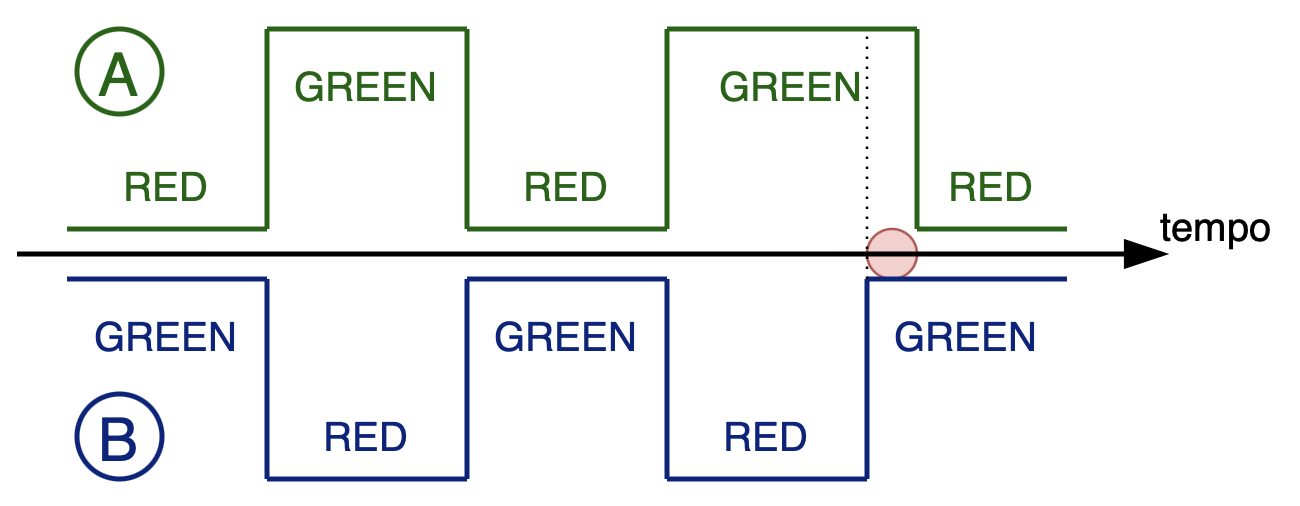
\includegraphics[width=0.7\linewidth]{figures/explicacaoSlots.png}
        \caption{Medição da precisão dos slots}
        \label{fig:explicacaoSlots}
    \end{figure}


    \begin{figure}[h]
      \begin{subfigure}{0.49\linewidth}
        \centering
        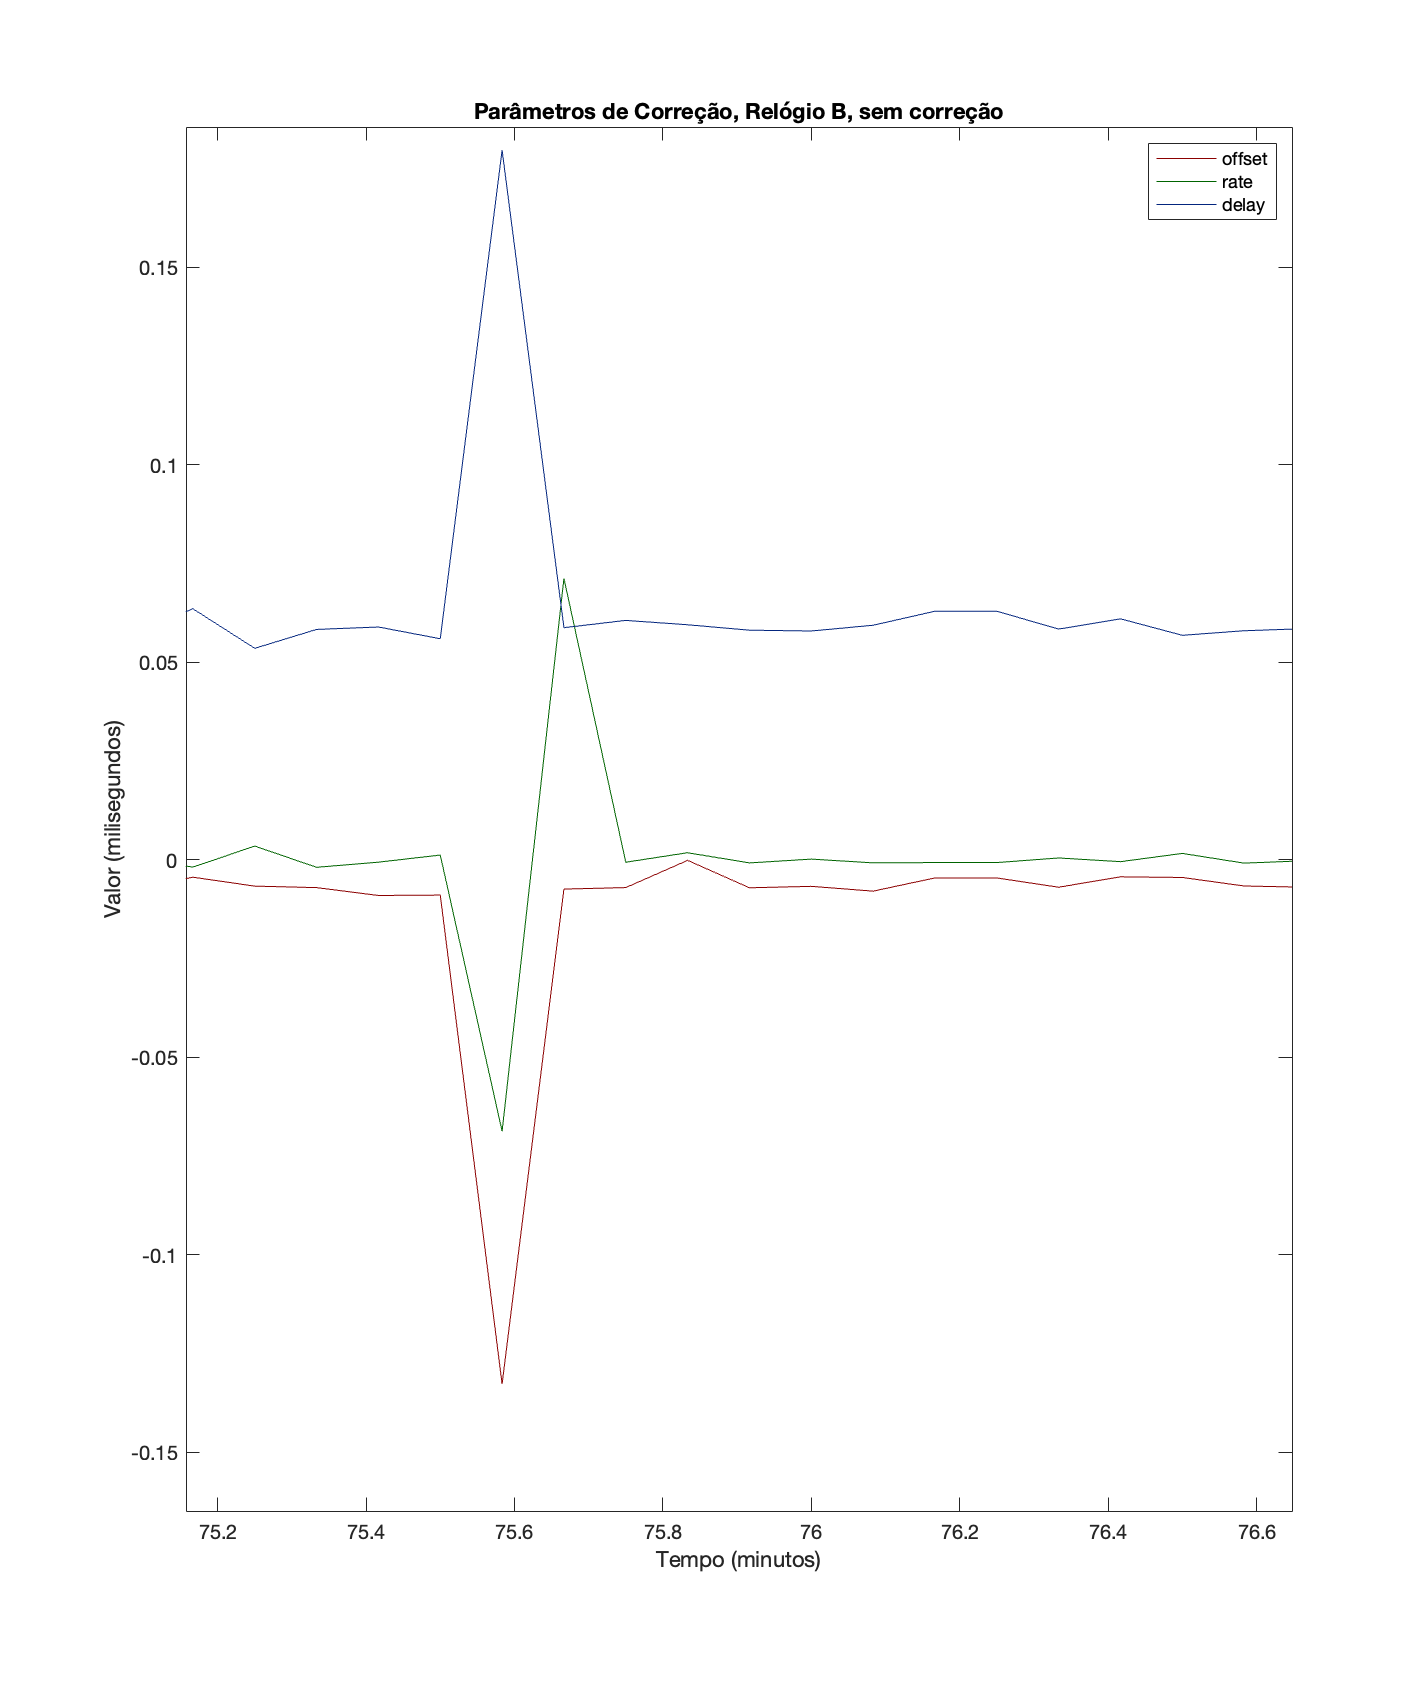
\includegraphics[width=\linewidth]{figures/rate_vs_delay_caso1.png}
        \caption{Rate sem considerar delay, sinal verde}
        \label{fig:rate_vs_delay_caso1}
      \end{subfigure}
      \begin{subfigure}{0.49\linewidth}
        \centering
        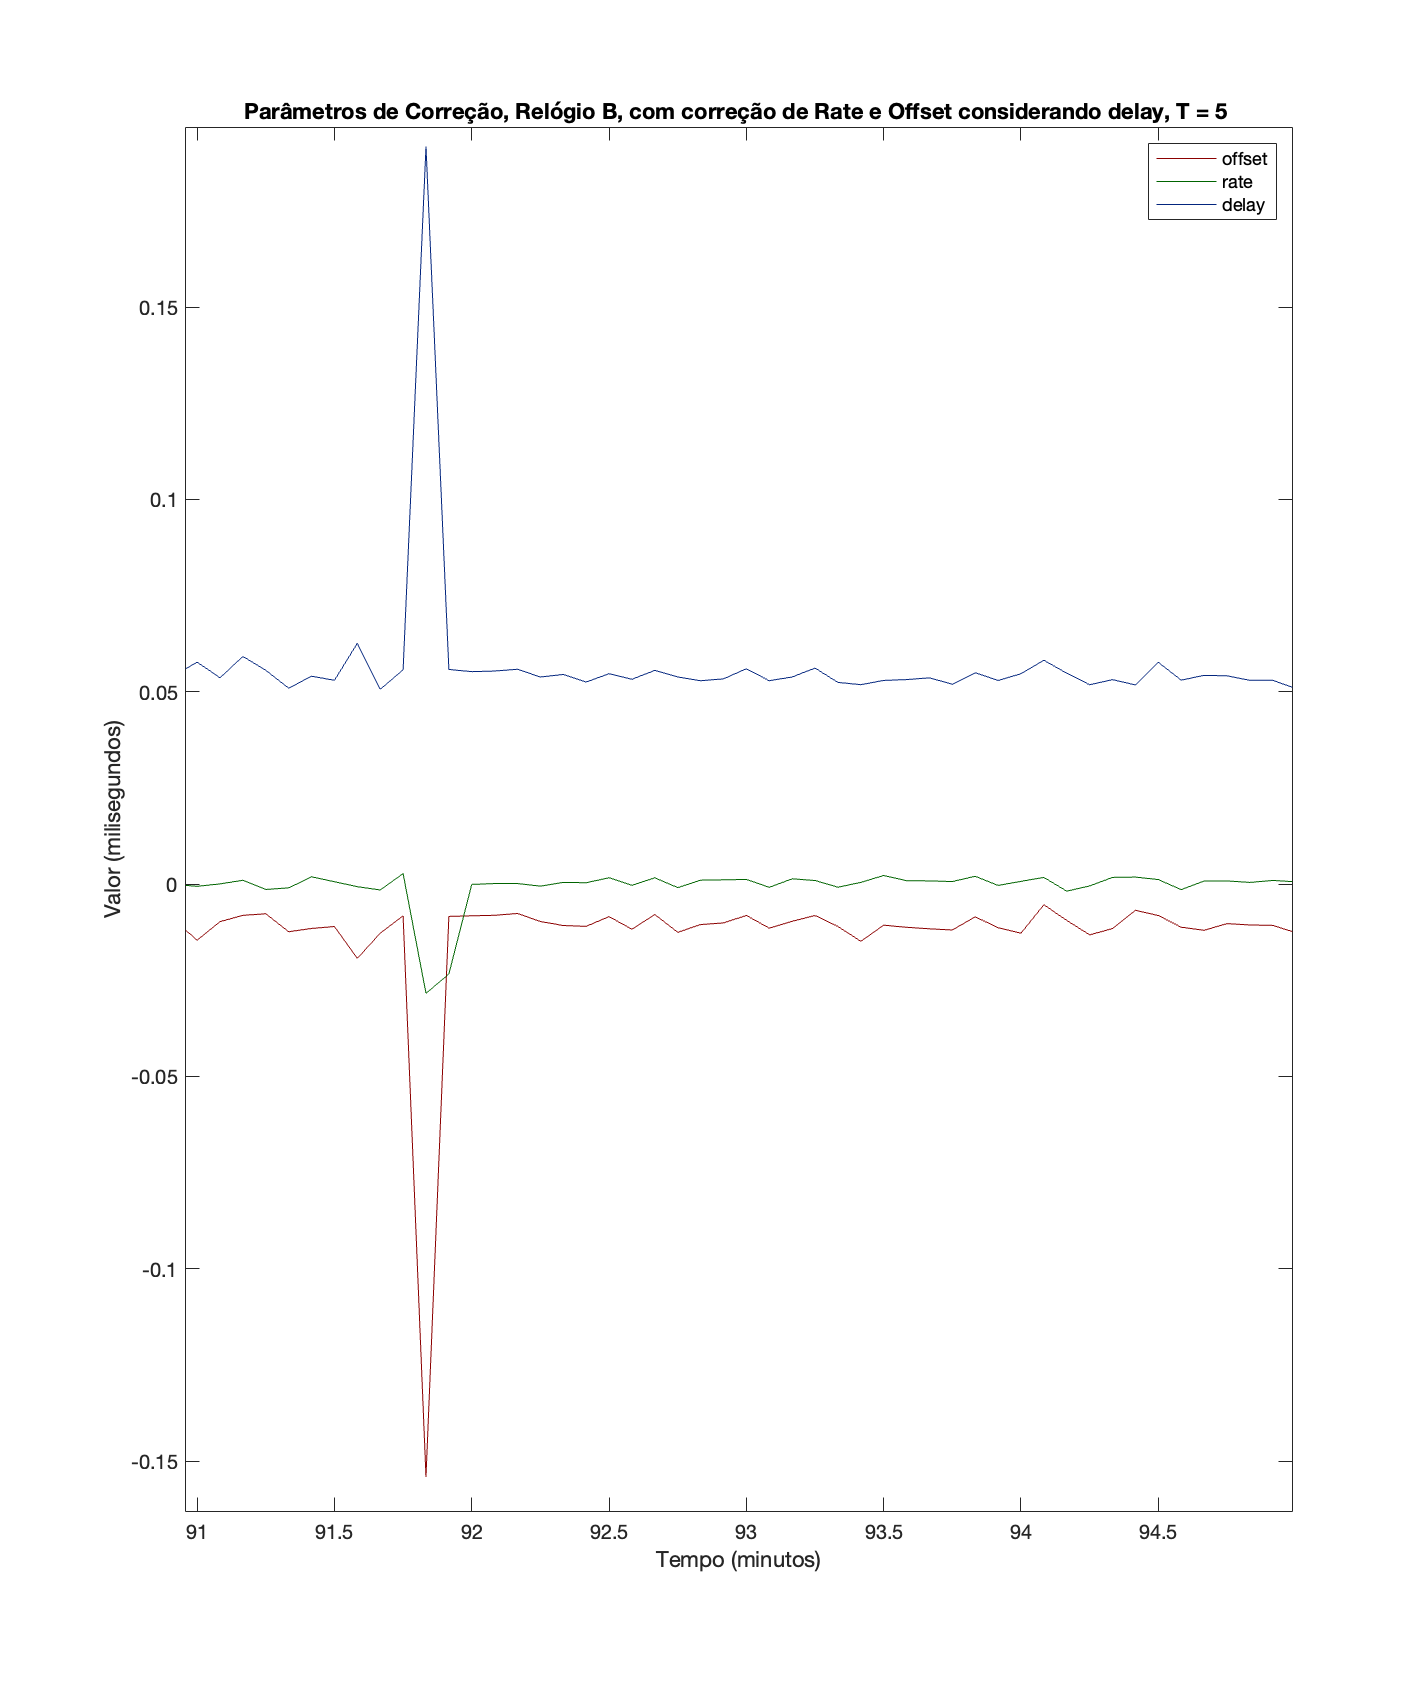
\includegraphics[width=\linewidth]{figures/rate_vs_delay_caso2.png}
        \caption{Rate considerando delay}
        \label{fig:rate_vs_delay_caso2}
      \end{subfigure}
    
      \caption{Influência da variação do delay no rate, sinal verde}
    \end{figure}
    
    \begin{figure}[h]
      \begin{subfigure}{0.49\linewidth}
        \centering
        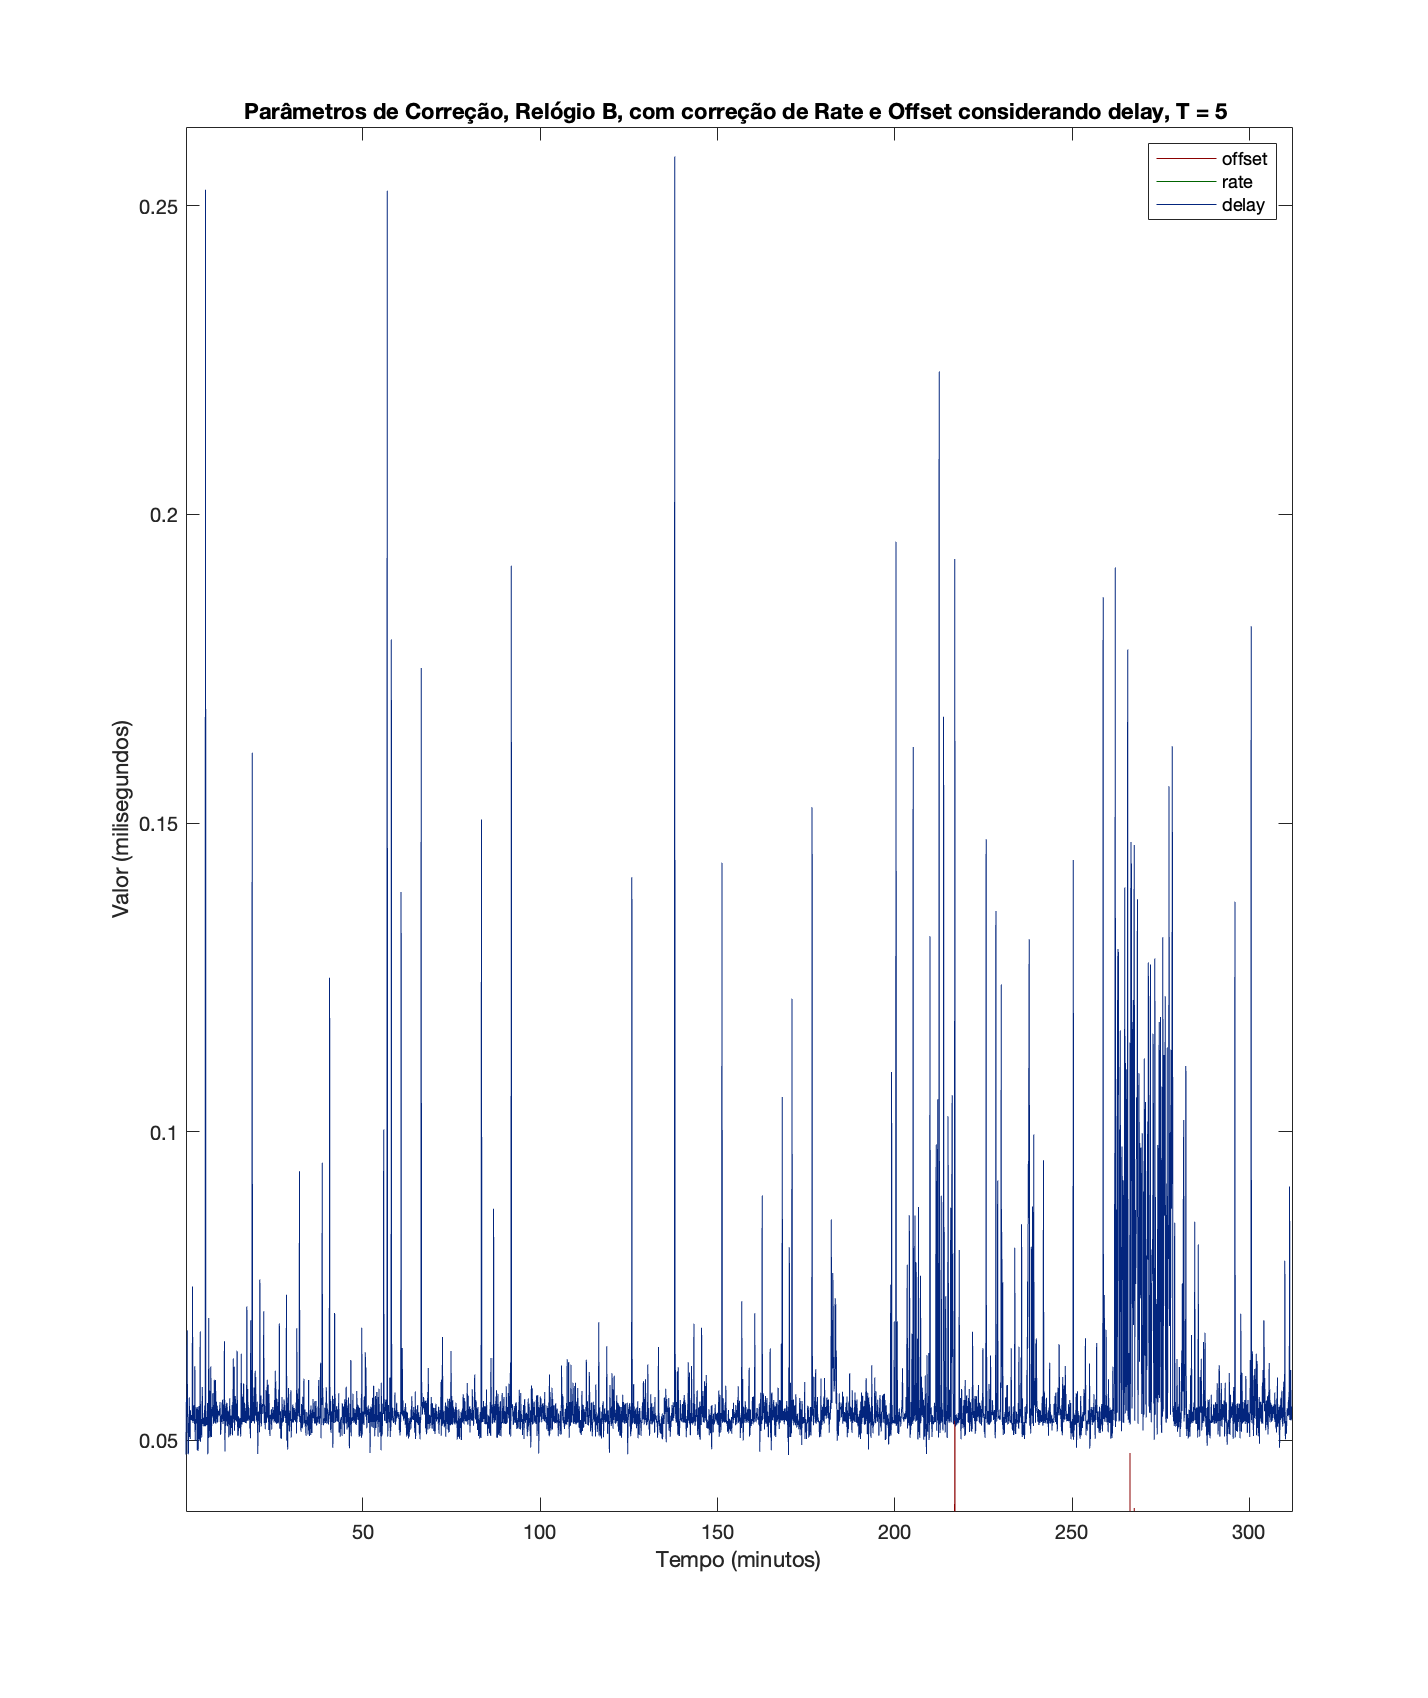
\includegraphics[width=\linewidth]{figures/delay.png}
        \caption{Variação do erro quadrático com o tempo}
        \label{fig:erroQuadratico}
      \end{subfigure}
      \begin{subfigure}{0.49\linewidth}
        \centering
        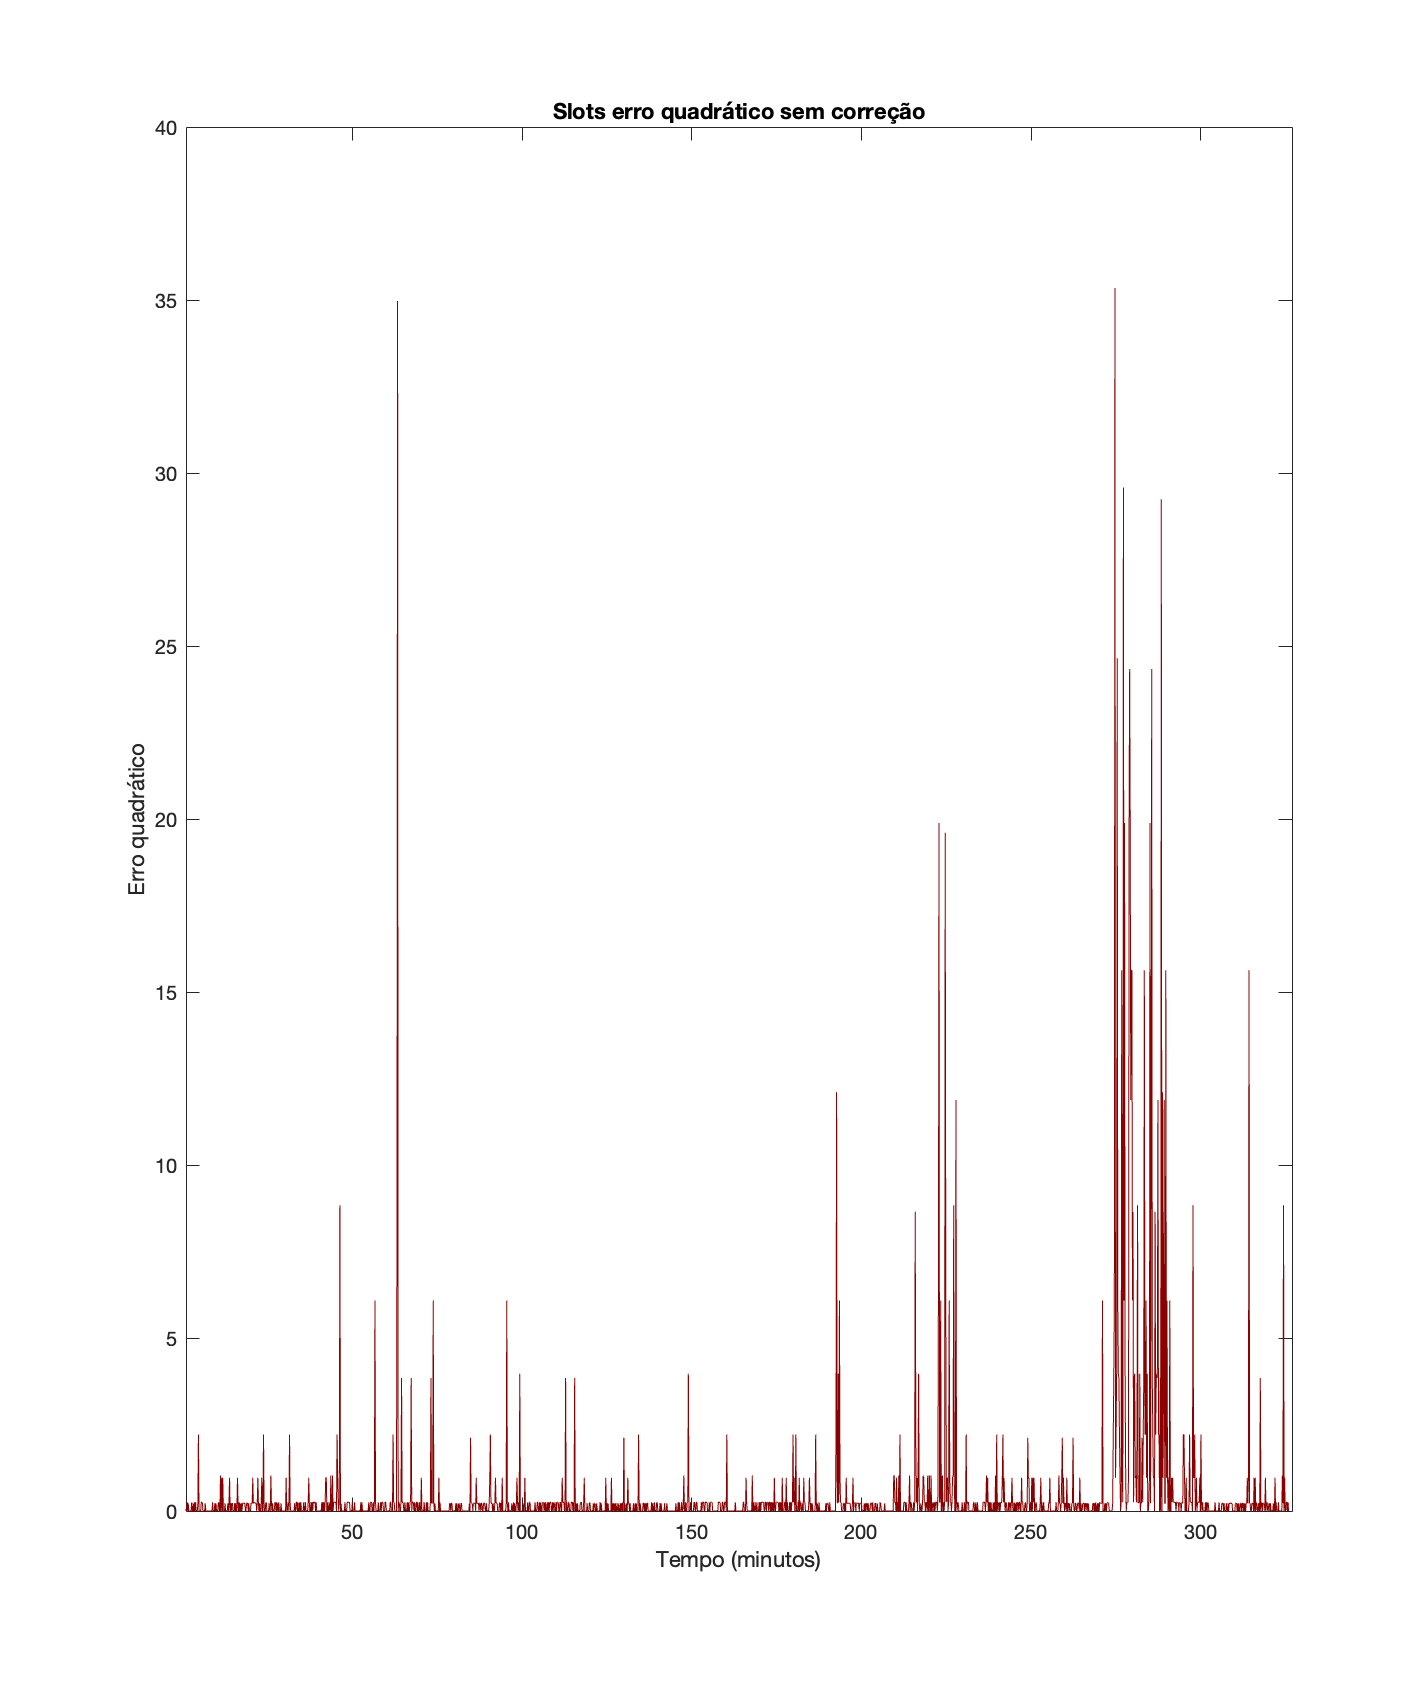
\includegraphics[width=\linewidth]{figures/erro_quadratico_delay.png}
        \caption{Variação do delay do servidor com o tempo}
        \label{fig:delay}
      \end{subfigure}
      \caption{Influência da variação delay no erro entre slots}
      \label{fig:delay_vs_erro}
    \end{figure}

    Por fim, a duração de cada experiência está presente na tabela \ref{tab:horas}, resultando num total de 34 horas e 15 minutos.
    
    \begin{table}[h]
\centering
\begin{tabular}{|c|c|c|c|c|c|}

\hline
 - & \makecell{S1 \\ T=5} & \makecell{S2 \\ T=5} & \makecell{S3 \\ T=5} & \makecell{S2 \\ T=2} & \makecell{S2 \\ T=15} \\ \hline
\makecell{Correção \\ rate}                  & 30  & 90   &  -  & -    & -    \\ \hline
\makecell{Correção \\ Rate + offset}         & 15  & 150  & 90  & 120  & 160  \\ \hline
\makecell{Correção \\ Rate + offset + delay} & 150 & 320  & 90  & 120  & 120  \\ \hline
\makecell{Sem \\ correção}                   & 600 & 600  & 600 & 600  & 600  \\ \hline
\end{tabular}
\caption{Duração de cada experiência, em minutos}
\label{tab:horas}
\end{table}

